\documentclass{article}


\usepackage{arxiv}

\usepackage[utf8]{inputenc} % allow utf-8 input
\usepackage[T1]{fontenc}    % use 8-bit T1 fonts
\usepackage{hyperref}       % hyperlinks
\usepackage{url}            % simple URL typesetting
\usepackage{booktabs}       % professional-quality tables
\usepackage{amsfonts}       % blackboard math symbols
\usepackage{nicefrac}       % compact symbols for 1/2, etc.
\usepackage{microtype}      % microtypography
\usepackage{lipsum}		% Can be removed after putting your text content
\usepackage{textgreek}
\usepackage{amsmath}
\usepackage{algorithm}
\usepackage{algpseudocode}
\usepackage{algpascal}
\usepackage{graphicx}
%\graphicspath{ {./images/} }

\title{Replicating Sutton's $TD(\lambda)$ Algorithm}

\date{June 1st, 2019}	% Here you can change the date presented in the paper title
%\date{} 					% Or removing it

\author{
  Carlos Souza\\
  %Department of Computer Science\\
  Georgia Institute of Technology\\
  São Paulo, SP, Brazil \\
  \texttt{souza@gatech.edu} \\
}

\begin{document}
\maketitle

\begin{abstract}
\lipsum[1]
\end{abstract}


% keywords can be removed
\keywords{First keyword \and Second keyword \and More}


\section{Introduction}
\label{sec:introduction}
Temporal-difference (TD) learning is a core learning technique in modern reinforcement learning  (Sutton, 1988; Kaelbling, Littman \& Moore; Sutton \& Barto, 1998; Szepesvári, 2014).
TD learning generates good estimates for expected returns by quickly bootstrapping from other expected-return estimates. TD($\lambda$) is one of the most popular algorithms in TD learning.
It was first introduced in Sutton's article \emph{Learning to Predict by the Methods of Temporal Differences}, one of the most referenced articles in the field with over 5,000 citations.
The purpose of this paper is to discuss the results obtained by replicating Sutton's TD($\lambda$) algorithm, providing a complete description of the experiments, implementation details and outcomes.

\subsection{Background}
\label{subsec:background}
Our focus in this paper are \emph{Markov Reward Processes}.
MRPs are stochastic processes that can be described by \(\langle\mathcal{S}, p, r, \gamma\rangle\), where \(\mathcal{S}\) is the set of all possible states, \(p(s'|s)\) is the transition probability from state \(s \in \mathcal{S}\) to state \(s' \in \mathcal{S}\), \(r(s, s')\) is the reward obtained in the transition, and \(\gamma\) is the discount factor.

We will also focus on episodic MRPs, processes that contain \emph{terminal states}.
These states divide the sequences of state transitions into \emph{episodes}.
Once a terminal state is reached, the episode ends and the state is reset to its initial value.
The return at time step \(t\) is the discounted sum of all the rewards observed after this time step until the end of the episode:

\begin{equation}
    G_{t} = \sum_{i=1}^{T-t} \gamma^{i-1} R_{i+1}\label{eqn:1}
\end{equation}

where \emph{T} is the time step of the terminal state.

Our goal is to learn the state-value function $v$ that maps each state $s \in \mathcal{S}$ to the expected return:

\begin{equation}
    v(s) = \mathbb{E}\{G_{t} \mid S_{t} = s\}\label{eqn:2}
\end{equation}

One of the simplest ways to solve a MRP is using Monte Carlo methods.
These methods solve reinforcement learning problems by using experience from interactions with the environment to update their estimate $V$ of $v$ for the nonterminal state $S_{t}$ ocurring in the experience.
Monte Carlo methods wait until the end of the episode, until the full return following the visit is known, to use this value to update current estimate of the state-value function:

\begin{equation}
    V(S_{t}) \leftarrow V(S_{t}) + \alpha(G_{t} - V(S_{t}))\label{eqn:3}
\end{equation}


where $\alpha$ is the learning-rate.
The problem with Monte Carlo methods is that $G_{t}$ is only known by the end of the episode, which means these methods must wait until the end of the episode to determine the increment to $V(S_{t})$.
TD methods, in other hand, need to wait only until the next step $t + 1$.
The simplest TD method, $TD(0)$, uses the observed reward $R_{t+1}$ and the current estimate $V(S_{t+1})$ from the next time step to update value-function estimate of current state:

\begin{equation}
    V(S_{t}) \leftarrow V(S_{t}) + \alpha \underbrace{(R_{t+1} + \gamma V(S_{t+1}) - V(S_{t}))}_{\delta \text{, known as TD error}} \label{eqn:4}
\end{equation}

$TD(0)$, also called \emph{one-step TD}, is just an instance of a more general class of algorithms called $TD(\lambda)$, where $\lambda = 0$.
The general $TD(\lambda)$ unify and generalize TD and Monte Carlo methods, producing methods that have Monte Carlo at one extreme ($\lambda = 1$) and one-step TD at the other ($\lambda = 0$).
Its update rule is similar to the $TD(0)$:

\begin{equation}
    V(S_{t}) \leftarrow V(S_{t}) + \alpha (R_{t+1} + \gamma V(S_{t+1}) - V(S_{t})) \: e(S_{t})\label{eqn:5}
\end{equation}

however, it is applied to \emph{all states} accordingly to their \emph{eligibility} $e(S_{t})$.
The eligibility of a state is the degree to which it has been visited in the past.
It is a short-term memory vector that is bumped in the component correspondent to the state recently visited, then fading away in proportion to $\lambda$.
Eligibility can be updated incrementaly as:

\begin{equation}
    e(s) \leftarrow \begin{cases}
                            \gamma \lambda \: e(s) + 1 &\text{if $s =$ current state}\\
                            \gamma \lambda \: e(s) &\text{otherwise}\label{eqn:6}
    \end{cases}
\end{equation}

We can use equations (\ref{eqn:5}) and (\ref{eqn:6}) to devise $TD(\lambda)$ algorithm:

\alglanguage{pseudocode}
\begin{algorithm}
    \caption{Value-state prediction with $TD(\lambda)$}
    \label{alg:1}
    \begin{algorithmic}
        \State Initialize state-value function $V$ arbitrarily
        \For{$episode \gets 1,\, M$}
            \State Initialize $S$
            \State Initialize $e$ to $0$ for all $s \in \mathcal{S}$
            \For{$t \gets 1,\, T$} \Comment{For each time step $t$ in the $episode$}
                \State Observe reward $R_{t+1}$ and next state $S_{t+1}$
                \State $e(S_{t}) \gets e(S_{t}) + 1$
                \State $\delta \gets R_{t+1} + \gamma V(S_{t+1}) - V(S)$
                \State $V(s) \gets V(s) + \alpha \: \delta \: e(s)$ for all $s \in \mathcal{S}$
                \State $e(s) \gets \gamma \: \lambda \: e(s)$ for all $s \in \mathcal{S}$
                \State $S_{t} \gets S_{t+1}$
            \EndFor
        \EndFor
    \end{algorithmic}
\end{algorithm}


\subsection{Random Walk}
\label{subsec:randomwalk}
Sutton (1988) illustrates TD methods with a random-walk example, one of the simplest dynamic systems.
A bounded random walk is a Markov Reward Process.
The episodes always start in the middle state $D$.
At each time step, the walk moves to the neighbor state, either left or right, with equal probability.
The episode ends when walk reaches either extreme states $A$ or $G$.
If termination happens by reaching the extreme right ($G$), environment provides a reward of +1;
all the other rewards are zero.

\begin{figure}[t]
    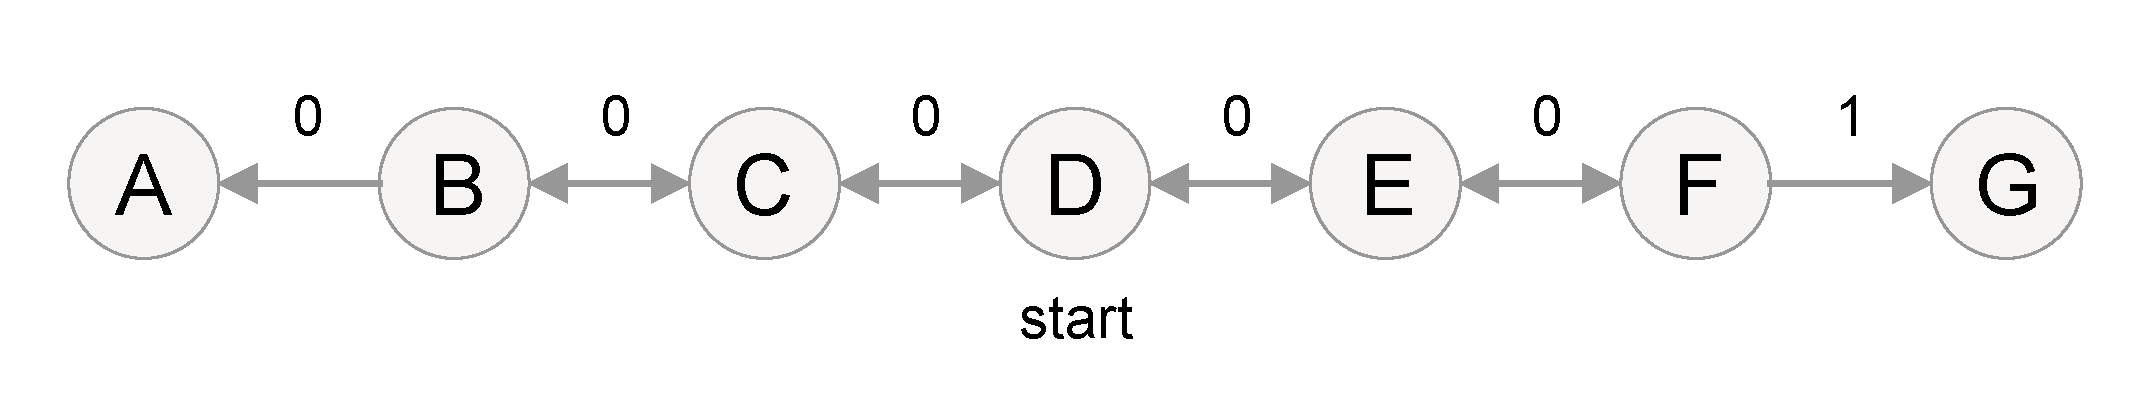
\includegraphics[scale=0.3]{./images/random_walk.eps}
    \centering
    \caption{A bounded random walk generator used in Sutton's original paper.
    All episodes start in state $D$.
    At each time step, walk has equal probability of either moving left or right.
    Episode ends when walk reaches either $A$ or $G$.
    In case of episode terminating in $G$, +1 reward is received;
    otherwise, reward is zero.}
    \label{fig:1}
\end{figure}

A typical episode terminating in the extreme right might be the following state-reward sequence: $D, 0, C, 0, D, 0, E, 0, F, 0, G, 1$.
An example of a walk ending in the extreme left might be: $D, 0, C, 0, B, 0, A, 0$.
This MRP is undiscounted ($\gamma = 1$);
therefore, the true value of each state is the probability of terminating on the extreme right by starting from that specific state.
Thus, the true values from all states, from $A$ to $G$ respectively, are

\begin{equation}
    v_{true} = \Bigg[0, \frac{1}{6}, \frac{2}{6}, \frac{3}{6}, \frac{4}{6}, \frac{5}{6}, 1\Bigg]
    \centering
\end{equation}

We applied $TD(\lambda)$ algorithm to effectively predict these true values, replicating Sutton's original paper methods and results.
The following sections explain in details how we implemented the experiments, their results, and compares them with the previously published outcomes.

\section{Methods}
\label{sec:methods}
To replicate Sutton's results, we followed the exact protocols described in the article.
First, we generated the data to be used by all learning procedures, by simulating 100 training sets, each containing 10 episodes (or sequences).
Then, we implemented the experiments using this data.
To measure how good the predictions were, we used the root mean squared (RMS) error between the predictions and the true values.

While implementing the experiments, we changed how the algorithm was written.
Sutton developed all the math in his paper and the algorithms considering that a prediction $P_{t}$ at time step $t$ is function of i) a vector $x_{t}$ of observations available at this time step (representing thus the state), and ii) a vector of modifiable weights, $w$.
This means he expressed all learning procedures and equations as rules for updating $w$.
However, the same learning procedures and equations can also be expressed as rules for updating state-value function $V$ directly, as $w = [V(S_{1}), V(S_{2}), V(S_{3}), ...]$, i.e. the vector in which each element is the state-value function $V(s)$ for each $s \in \mathcal{S}$.
As the underlying math is exactly the same, we arrived at the same results and conclusions, as we will show in the next section.

The first experiment assessed how different values of $\lambda$ produced different predictions with different corresponding RMS errors.
We used $\lambda = 0, 0.1, 0.3, 0.5, 0.7, 0.9$ and $1$.
There are 2 special cases in these values: 0 and 1.
$TD(0)$ is the \emph{one-step} TD, which updates the value-function using the reward from only one step ahead.
$TD(1)$ is an instance of the Monte Carlo methods, which updates value-function only after the episode is complete, using all the rewards until the end of the episode.
This case of $\lambda = 1$ is also referred as Widrow-Hoff in the original paper.

In this experiment, the state-value function was not updated neither online (i.e. after each time step, as shown in the algorithm \ref{alg:1}) nor by the end of each episode.
Instead, the function was only updated after a full loop over all episodes in the training set.
Also, following the paper, we implemented the \emph{repeated presentations} training paradigm in this experiment: we executed the training loop for each training set repeatedly, using the same data, until the state-value function did not change significantly.
Here the paper is unclear about: i) the learning rate ($\alpha$) used, ii) how to assess significant changes in the state-value function throughout the simulation, and iii) the minimum threshold difference between different estimates of state-value functions, below which the simulation ends.
We used $\alpha = 0.01$ (as the paper mentions it used a small learning rate to ensure conversion), RMS error as a way to assess with a single scalar the difference between two estimates of value-functions, and $\theta = 10^{-4}$ as threshold to stop the simulation: whenever the RMS error between two estimates of different value-functions fall below this, the simulation ends.

In the second experiment we simulated different values of $\alpha$ and different values of $\lambda$, to understand the impact of the learning rate in TD.
Three important changes were made in comparison to the first experiment.
First, the training loop was executed only once for each training set.
Second, the state-value function was updated by the end of each episode.
Third, different than the first experiment, where the state-value function was initialized randomly, now the state-value function was initialized at constant value of $0.5$ for all states.
We varied $\alpha$ from $0$ to $0.6$ in steps of $0.05$, and $\gamma$ from $0$
 to $1$ in steps of $0.1$.


\section{Results}
\label{sec:results}

\begin{figure}[t]
    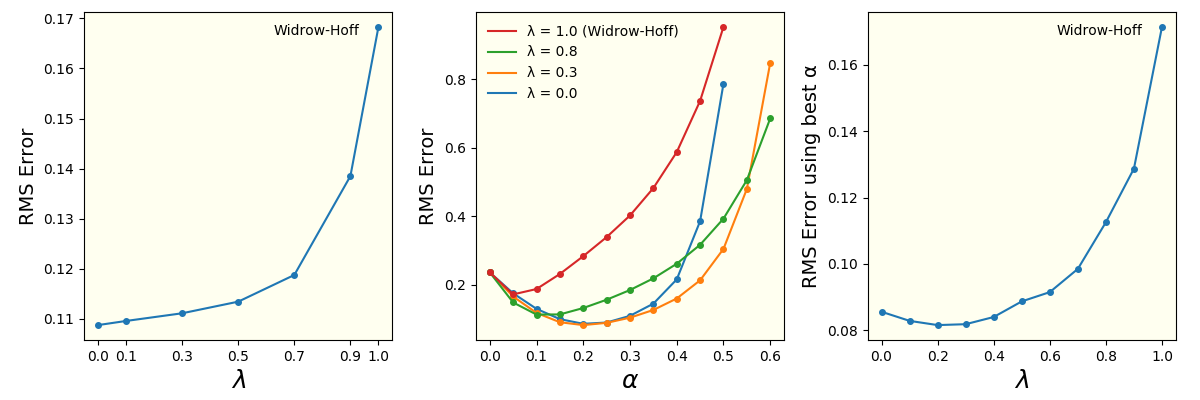
\includegraphics[width=\textwidth]{./images/figure.png}
    \centering
    \label{fig:fig2}
    \caption{Replication of Figures 3, 4 and 5 from Sutton's original paper.
    In the left, average error on random walk problem under repeated presentations.
    In the center, average error on random walk problem after 10 episodes for different values of $\alpha$ and $\gamma$.
    In the right, average error at best $\alpha$ on random walk problem for different values of $\gamma$.}
\end{figure}

Figure 2 summarizes the results obtained by replicating Sutton's experiments.
In the left, the chart shows the results of the first experiment, where RMS errors were calculated between the state-value function true values and the ones estimated after repeated presentations until convergence, for different values of $\lambda$.
We averaged the errors over 100 training sets, exactly as done by Sutton.
This chart replicates Figure 3 in the original article.

In the center, the chart shows average errors obtained in a single run of each training set, averaged over 100 training sets, for different values of $\alpha$ and $\lambda$
This chart replicates Figure 4 in the original article.

Finally, in the right, we can see the chart that replicates Figure 5 in Sutton's article.
The results were produced by experiment 2, after a single run of each training set, also averaged over 100 training sets, for different values of $\alpha$ and $\lambda$.
For each value of $\lambda$, we selected the best value of $\alpha$.

As we can see, our results matched the overall results obtained by Sutton.
In the next section we will discuss in details the similarities, the small diferences, and explain why these results were expected.


\section{Discussion}
\label{sec:discussion}
\lipsum[2]
\lipsum[3]

\lipsum[2]
\lipsum[3]


\section{Conclusion}
\label{sec:conclusion}
\lipsum[2]
\lipsum[3]


\bibliographystyle{unsrt}
\bibliography{references}  %%% Remove comment to use the external .bib file (using bibtex).
%%% and comment out the ``thebibliography'' section.


\end{document}
